\documentclass[11pt,a4paper]{article}

% Packages
\usepackage[utf8]{inputenc}
\usepackage[spanish, es-tabla, es-lcroman]{babel}
\usepackage{caption}
\usepackage{listings}
\usepackage{adjustbox}
\usepackage[shortlabels]{enumitem}
\usepackage{boldline}
\usepackage{amssymb, amsmath}
\usepackage[margin=1in]{geometry}
\usepackage{xcolor, color}
\usepackage{soul}
\usepackage{epstopdf}
\usepackage{hyperref}
\hypersetup{
     colorlinks   = true,
}

% Meta
\title{\textbf{ESTRUCTURA DE DATOS}\\
	   \textit{Práctica 1. Eficiencia de algoritmos}\\
	   \large \vspace{0.25em} Doble Grado de Informática y Matemáticas}
\author{Víctor Castro Serrano\\ Maximino Suárez van Gelderen}
\date{\today}

% Custom
\providecommand{\abs}[1]{\lvert#1\rvert}
\setlength\parindent{0pt}
\definecolor{Light}{gray}{.90}
\definecolor{mygreen}{rgb}{0,0.6,0}
\definecolor{mygray}{rgb}{0.5,0.5,0.5}
\definecolor{mymauve}{rgb}{0.58,0,0.82}
\renewcommand\labelenumi{(\emph{\roman{enumi})}}
\newcommand{\bm}[1]{\boldsymbol{#1}}

\lstset{literate=   % listings config
  {á}{{\'a}}1 {é}{{\'e}}1 {í}{{\'i}}1 {ó}{{\'o}}1 {ú}{{\'u}}1
  {Á}{{\'A}}1 {É}{{\'E}}1 {Í}{{\'I}}1 {Ó}{{\'O}}1 {Ú}{{\'U}}1
  {à}{{\`a}}1 {è}{{\`e}}1 {ì}{{\`i}}1 {ò}{{\`o}}1 {ù}{{\`u}}1
  {À}{{\`A}}1 {È}{{\'E}}1 {Ì}{{\`I}}1 {Ò}{{\`O}}1 {Ù}{{\`U}}1
  {ä}{{\"a}}1 {ë}{{\"e}}1 {ï}{{\"i}}1 {ö}{{\"o}}1 {ü}{{\"u}}1
  {Ä}{{\"A}}1 {Ë}{{\"E}}1 {Ï}{{\"I}}1 {Ö}{{\"O}}1 {Ü}{{\"U}}1
  {â}{{\^a}}1 {ê}{{\^e}}1 {î}{{\^i}}1 {ô}{{\^o}}1 {û}{{\^u}}1
  {Â}{{\^A}}1 {Ê}{{\^E}}1 {Î}{{\^I}}1 {Ô}{{\^O}}1 {Û}{{\^U}}1
  {œ}{{\oe}}1 {Œ}{{\OE}}1 {æ}{{\ae}}1 {Æ}{{\AE}}1 {ß}{{\ss}}1
  {ű}{{\H{u}}}1 {Ű}{{\H{U}}}1 {ő}{{\H{o}}}1 {Ő}{{\H{O}}}1
  {ç}{{\c c}}1 {Ç}{{\c C}}1 {ø}{{\o}}1 {å}{{\r a}}1 {Å}{{\r A}}1
  {€}{{\EUR}}1 {£}{{\pounds}}1 {ñ}{{\~{n}}}1
}

\lstset{    %listings config
  language=C++,
  belowcaptionskip=1\baselineskip,
  breaklines=true,
  frame=L,
  xleftmargin=0.5in,
  %otherkeywords={},
  showstringspaces=false,
  backgroundcolor=\color{white},
  basicstyle=\footnotesize\ttfamily,
  keywordstyle=\bfseries\color{purple!90!black},
  commentstyle=\itshape\color{gray!85!},
  identifierstyle=\color{blue!80!black},
  stringstyle=\color{green!60!black},
}

\newcommand\ddfrac[2]{\frac{\displaystyle #1}{\displaystyle #2}}

% Environments

\begin{document}
\maketitle

\section*{Condiciones de ejecución.}

Dado que en los siguientes ejercicios hablaremos de la eficiencia de distintos programas, conviene detallar las condiciones en las que se han llevado a cabo las pruebas. \\

\textbf{Hardware:} Asus GL552VW, Intel Core i5-6300HQ CPU @ 2.30GHz 4 cores, Intel HD Graphics 530 (Skylake GT2), 12GB RAM. \\
\textbf{Sistema Operativo:} Ubuntu 16.04.3 LTS 64-bit. \\
\textbf{Compilador:} g++ \\
\textbf{Opciones de compilación:} -g -o

\section*{Ejercicio 1.}
En este ejercicio, comprobaremos tanto la eficiencia teórica como la eficiencia empírica del algoritmo de ordenación \emph{burbuja}:

\begin{lstlisting}[numbers=left]
void ordenar(int *v, int n)
{
  for (int i=0; i<n-1; i++)
    for (int j=0; j<n-i-1; j++)
      if (v[j]>v[j+1]) {
        int aux = v[j];
        v[j] = v[j+1];
        v[j+1] = aux;
      }
}
\end{lstlisting}

Comencemos analizando la eficiencia teórica del algoritmo, en el caso peor. Veamos primero el coste en operaciones elementales (OE) de cada línea:\\

\textbf{Línea 3.} Hay 4 OE: una asignación, una resta, una comparación y un incremento.

\textbf{Línea 4.} Hay 5 OE: igual que la línea anterior, pero se realizan dos restas.

\textbf{Línea 5.} Hay 4 OE: dos accesos a un vector, una suma y una comparación.

\textbf{Línea 6.} Hay 2 OE: asignación y acceso al vector.

\textbf{Línea 7.} Hay 4 OE: dos accesos, suma y asignación.

\textbf{Línea 8.} Hay 3 OE: acceso, suma y asignación.\\

Entonces, la eficiencia del algoritmo es:

$$ T(n) = \sum_{i=0}^{n-2} \left( 4 + \sum_{j=0}^{n-i-2} 4+9 \right) =  \sum_{i=0}^{n-2} \left( 4 + 13(n-i-1) \right) =  \frac{13n^{2}-5n-8}{2}.$$

Por tanto, afirmamos que $T(n) \in O(n^2)$, y el algoritmo de ordenación burbuja es de orden de eficiencia $O(n^2)$.\\

Ahora creamos un programa de prueba para analizar la eficiencia empírica, haciendo uso de la biblioteca \emph{ctime} del lenguaje C++:

\lstinputlisting{ordenacion.cpp}

Al analizar la eficiencia empírica del algoritmo, obtenemos la siguiente gráfica:\\

\begin{center}
	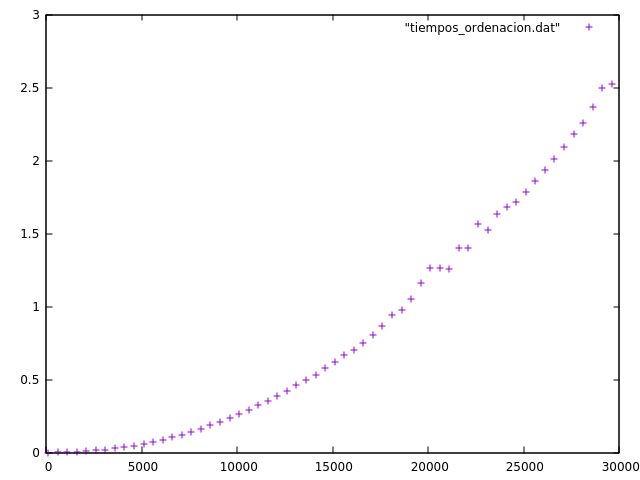
\includegraphics[height=7cm]{graficaej1.png}
\end{center}

Si representamos superpuestas la función de la eficiencia teórica y la empírica, obtenemos lo siguiente:\\

\begin{center}
	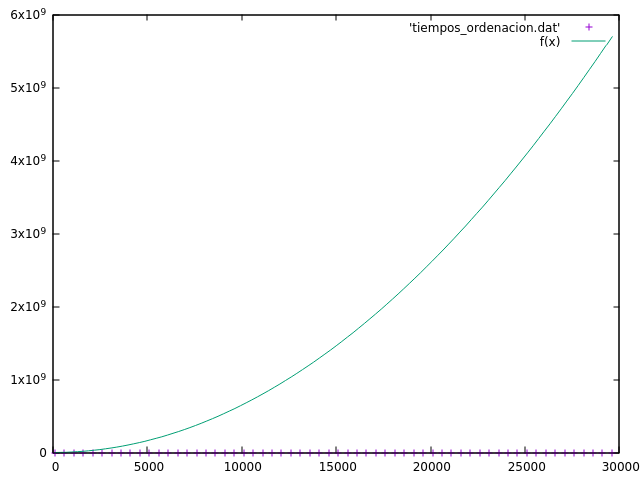
\includegraphics[height=7cm]{teorica-empirica.png}
\end{center}

Observamos que, aunque la curva de la eficiencia teórica tiene la misma forma que la nube de puntos obtenidas experimentalmente, ambas curvas no coinciden al representarlas superpuestas. Esto se debe a que las constantes no coinciden, pues el costo de una operación elemental, e incluso el tiempo total de ejecución del algoritmo, dependen de las condiciones particulares de la máquina en la que se ejecuta.

\end{document}
